\chapter{Diseño detallado}\label{cap8}

Posterior a la selección del diseño conceptual que más se adecua a las
necesidades del usuario y su importancia relativa, se procedió con el diseño
detallado del sistema, en el cual se documentan los cálculos, selección de
componentes y justificaciones teóricas que rigen la geometría del tanque.

El objetivo fue crear las especificaciones técnicas necesarias para la 
fabricación, ensamblaje y automatización del sistema. El diseño detallado se
desglosará en los siguientes puntos:

\begin{enumerate}
  \item \textbf{Diseño Geométrico y Mecánico:} Justifica la geometría del tanque principal.
  \item \textbf{Selección de componentes:} En esta sección se detallan las características que fueron determinantes al seleccionar los componentes que conformarán el sistema.
  \item \textbf{Integración y CAD:} Se describe la disposición de los elementos hidráulicos y neumáticos, sistema de iluminación e interfaz.
  \item \textbf{Sistema de Control:} Describe la arquitectura de control, incluye el proceso de diseño de los diferentes tipos de control que se utilizarán en el proyecto.
  \item \textbf{Programación:} Detalla el algoritmo utilizando, haciendo uso los diagramas de flujo con la estructura del código que rige el comportamiento del sistema.
  \item \textbf{Sistemas Eléctricos:} Presenta los esquemas de conexión y la integración de los componentes electrónicos como actuadores, sensores y microcontroladores.
  \item \textbf{Plan de manufactura:} Define la ruta de fabricación, la selección de herramientas y los procesos técnicos de montaje.
\end{enumerate}

\section{Diseño geométrico y mecánico}

\subsection{Dimensiones y estructura del biorreactor}

El cultivo de hongos filamentosos en biorreactores convencionales presenta
algunas desventajas, entre ellas la adhesión de micelio en las paredes, la baja
resistencia del hongo a fuerzas cortantes, necesidad de un entorno homogéneo y
altas tasas de transferencia de oxígeno. La geometría propuesta en este diseño
busca atacar estas debilidades mediante la adecuación de las dimensiones a las
necesidades propias del organismo y la incorporación de elementos nuevos.

La configuración de biorreactor tipo airlift (Figura~\ref{fig:airlift_config}) mitiga el estrés por
cizallamiento, puesto que elimina los elementos mecánicos de agitación. Esta
configuración se caracteriza por la inyección de gas en la parte inferior y un aro que
conduce el flujo. El flujo es resultado de la diferencia de densidad entre dos
regiones, a la región donde se inyecta el gas se le denomina \textit{riser}, mientras que la
zona donde el fluido recircula hacia la base se llama \textit{downcomer} \cite{Cerrone2024}.

\begin{figure}[H]
  \centering
  
\includegraphics[width=0.3\textwidth]{airlift_configuracion}
  \caption{Configuración de un biorreactor tipo airlift \cite{Cerrone2025}.}
  \label{fig:airlift_config}
\end{figure}

La configuración convencional mostrada en la Figura~\ref{fig:airlift_config}, tiene la desventaja de que
requiere una distancia considerable entre nivel de agua y superficie (espacio libre
superior) para asegurar el flujo \cite{Cerrone2025}, sin embargo, la existencia de esta área libre
promueve la formación de micelio. Siguiendo el mismo principio, se han
desarrollado diferentes modificaciones, entre ellas el biorreactor airlift con aro
externo, el cual al contar con una separación física entre \textit{riser} y \textit{downcomer}, no
cuenta con la limitante de que el flujo esté relacionado con el área libre superior.
Además, el espacio que permitiría la recirculación interna se aprovechará para la
incorporación del sistema de iluminación. La Figura~\ref{fig:partes_airlift} muestra el diseño tipo airlift
con aro externo.

\begin{figure}[H]
  \centering
  
\includegraphics[width=0.6\textwidth]{airlift_partes}
  \caption{Partes de un biorreactor tipo airlift con aro externo.}
  \label{fig:partes_airlift}
\end{figure}

Existen algunas relaciones estandarizadas para biorreactores cilíndricos
(preferidos para evitar el estancamiento). Se prefieren biorreactores con una
relación entre la altura total ($H$) y diámetro interno del tanque
($D$) de entre 3 y 15 para facilitar el flujo. En esta ocasión la
relación $H/D$ se mantuvo en aproximadamente 5.08 ($H $= 1\,093~mm, $D$ = 215~mm),
esto debido al aumento del diámetro del tanque para alojar el tubo de tiro concéntrico
con el sistema de iluminación integrado \cite{Moresi2025}.

Otra relación encontrada en la bibliografía es el área de la sección transversal del
\textit{downcomer} ($A_d$, conducto de descenso) con respecto a la del \textit{riser} ($A_r$, columna de
ascenso y oxigenación) de 0.5 a 1 para aumentar la velocidad de transferencia. En
esta ocasión, se obtuvo una relación $A_d/A_r$ = 0.201, donde la mayor parte del volumen
de cultivo se distribuye en la zona anular del \textit{riser}, iluminada desde el centro
por el sistema integrado en el interior del tubo de tiro. En el Anexo~\ref{ap:estructura} se contienen los cálculos para la geometría
del reactor.

Siempre que existen curvaturas en el tanque, la norma ASME BPE sugiere
mantener ciertas relaciones para facilitar la limpieza CIP del tanque. Este estándar
define las dimensiones precisas para los accesorios higiénicos utilizados en estas
aplicaciones. Para el diseño de las líneas de tubería de 96.52~mm, equivalente nominal
a 3.8 pulgadas, se ha consultado la Tabla \ref{fig:radio_curvatura} (Anexo~\ref{ap:estructura}) extraída de dicha norma. De acuerdo con esta
tabla, para un tamaño de tubería nominal de 4 pulgadas el estándar BPE especifica
un radio de curvatura de 6 pulgadas \cite{Huitt2016}.

La Tabla~\ref{tab:medidas_tanque} recopila las dimensiones seleccionadas para la generación de la
geometría del tanque.

\begin{table}[H]
\centering
\caption{Tabla recopiladora de medidas del tanque.}
\label{tab:medidas_tanque}
\renewcommand{\arraystretch}{1.3}
\small
\begin{tabularx}{\textwidth}{@{} X l l @{}}
\toprule
\textbf{Nombre} & \textbf{Designación} & \textbf{Valor} \\
\midrule
Radio interno del tanque (\textit{riser}) & $R_r$ & 107.5~mm \\
Radio interno del tubo de tiro (\textit{downcomer}) & $R_d$ & 48.26~mm \\
Altura de la zona de cultivo & $H$ & 1093~mm \\
Altura del tubo de tiro  & $H_d$ & 670.2~mm \\
Radio de curvatura       & $R_B$ & 152.4~mm \\
Capacidad volumétrica total del tanque & $V$ & 55~L \\
\bottomrule
\end{tabularx}
\end{table}

\begin{figure}[H]
  \centering
  
\includegraphics[width=0.6\textwidth]{simbologia_geometria}
  \caption{Simbología de los parámetros utilizados para la geometría del biorreactor.}
  \label{fig:simbologia}
\end{figure}
Una vez obtenidos estos parámetros, se realizó el modelo CAD del tanque final, en el cual se incorporaron divisiones para asegurar la modularidad del contenedor y facilitar su limpieza.
Todas las uniones contemplan su respectiva brida de sujección, ranura y o-ring; las dimensiones de las ranuras para o-ring se detallan en el Anexo~\ref{ap:estructura}.
Al modelo se le incorporaron también las roscas que conectan el tanque con los accesorios exteriores, para ello se utilizó roscado NPT \footnote{National Pipe Thread Taper (NPT): estándar estadounidense de rosca cónica para tuberías, utilizado en conexiones de líquidos, gases, vapor y fluidos hidráulicos.}. 
El modelo CAD con todos los elementos mencionados en esta sección se presenta en la Figura~\ref{fig:solotanque}.
\begin{figure}[H]
	\centering
	
\includegraphics[width=0.6\textwidth]{CAD_tanque}
	\caption{Diseño CAD para tanque del biorreactor.}
	\label{fig:solotanque}
\end{figure}

Los planos de fabricación del biorreactor con acotado completo se presentan en el Anexo~\ref{ap:planos}.

\subsection{Análisis de esfuerzos y validación estructural}

Para corroborar la integridad física del biorreactor ante las condiciones de operación esperadas, se realizó un análisis de elemento finito (FEA). Se evaluaron dos escenarios: la presión hidrostática del medio de cultivo y la presión manométrica ante la inyección de aire.

Se considera una estructura fabricada en acero inoxidable AISI~304 (18-8), material ampliamente utilizado en la industria alimentaria y biotecnológica debido a su inocuidad y resistencia a la corrosión~\cite{Serviacero}; además de un espesor de pared de 3.5~mm para el tanque.

Para el análisis hidrostático se consideraron la densidad del medio y la aceleración gravitacional, arrojando un factor de seguridad mínimo de 91.1, demostrando que el contenedor soporta el peso del líquido con un margen de seguridad considerable.

En tanto al análisis de la presión manométrica, se sometió al modelo a una carga de 0.50~MPa (5~bar) para evaluar su comportamiento ante fallas en las válvulas de alivio, donde se obtuvo un factor de seguridad mínimo de 3.18, superando el criterio de diseño FS~$\geq 2$.

El Anexo~\ref{ap:estructura} reúne el proceso de simulación del comportamiento del modelo ante las cargas expresadas, así como los resultados obtenidos.

\subsection{Selección de pernos}

Para garantizar la integridad hermética y estructural del biorreactor ante una presión interna de 5~bar, se realizó un análisis de fatiga y precarga en los pernos de sujeción. El diseño utiliza una configuración de 8~pernos $\tfrac{5}{16}$-18~UNC, SAE Grado~5, distribuidos en un diámetro de sellado de 170~mm.

Se utilizó el modelo de rigidez de juntas de Shigley para determinar el factor de seguridad a la fluencia, carga y separación de la unión. El Anexo~\ref{ap:estructura} recopila los cálculos efectuados, mientras que la Tabla~\ref{tab:factores_seguridad} recopila los resultados de seguridad obtenidos.

\begin{table}[H]
\centering
\caption{Tabla de los resultados de los factores de seguridad.}
\label{tab:factores_seguridad}
\renewcommand{\arraystretch}{1.3}
\small
\begin{tabular}{llcc}
\toprule
\textbf{Factor de seguridad} & \textbf{Símbolo} & \textbf{Valor obtenido} & \textbf{Criterio de aceptación} \\
\midrule
A la fluencia                & $n_p$ & 1.281 & $> 1$ \\
A la carga                   & $n_L$ & 8.133 & $> 1$ \\
A la separación de la unión  & $n_0$ & 6.836 & $> 1.2$ (\textit{para evitar fugas}) \\
\bottomrule
\end{tabular}
\end{table}

\section{Selección de componentes}

\subsection{Raspberry Pi (4B)}

El control del biorreactor requiere la ejecución simultánea de la adquisición de datos de los diferentes sensores, activación de actuadores, manipulación de lazos de control PI y difuso, así como la actualización constante del interfaz humano-máquina. Por ello se seleccionó la Raspberry Pi 4B, ya que su arquitectura permite la gestión de múltiples tareas. Además de contar con soporte para protocolos de video, permite el uso de tarjetas microSD, por lo que se podrá contar con una base de datos local y facilita su exportación. Otra de las ventajas es el lenguaje de programación, puesto que al trabajar con Qt/QML y C++ se facilita el desarrollo de la interfaz. La Figura~\ref{fig:raspberry} muestra el microprocesador seleccionado mientras que en la Tabla~\ref{tab:raspberry} se muestran sus características más importantes.

\begin{figure}[H]
  \centering
  
\includegraphics[width=0.5\textwidth]{raspberry_4b}
  \caption{Raspberry Pi (4B).}
  \label{fig:raspberry}
\end{figure}

\begin{table}[H]
\centering
\caption{Tabla descriptiva de Raspberry Pi (4B).}
\label{tab:raspberry}
\renewcommand{\arraystretch}{1.3}
\small
\begin{tabularx}{\textwidth}{@{} l X @{}}
\toprule
\textbf{Parámetro} & \textbf{Valor} \\
\midrule
Descripción    & Procesador de cuatro núcleos a 1.5~GHz, 1~GB de RAM LPDDR4, Gigabit Ethernet, Wifi de doble banda y dos puertos micro-HDMI. \\
Voltaje        & 5~V DC \\
Corriente      & 3~A \\
Potencia       & 25~W \\
Memoria        & 2~GB \\
Almacenamiento & 128~GB \\
\bottomrule
\end{tabularx}
\end{table}

\subsection{Sensor de oxígeno y temperatura RK500-04 Tipo-B}

El sensor de oxígeno y temperatura RK500-04 fue seleccionado debido a su alta confiabilidad, material biocompatible y características eléctricas y de comunicación adaptables al sistema planteado. Dado que la oxigenación es un factor determinante para asegurar la vida del organismo, es requerido contar con una medición fiel en todo momento. Se escogió este modelo entre otras opciones más económicas principalmente por el material de grado alimenticio y su alta resolución, la cual permite mediciones más precisas. La Figura~\ref{fig:sensor_od} muestra el sensor seleccionado mientras que en la Tabla~\ref{tab:sensor_od} se muestran sus características más importantes.

\begin{figure}[H]
  \centering
  
\includegraphics[width=0.5\textwidth]{sensor_od_rk500}
  \caption{Sensor de oxígeno disuelto y temperatura RK500-04.}
  \label{fig:sensor_od}
\end{figure}

\begin{table}[H]
\centering
\caption{Tabla descriptiva de sensor RK500-04.}
\label{tab:sensor_od}
\renewcommand{\arraystretch}{1.3}
\small
\begin{tabularx}{\textwidth}{@{} l X @{}}
\toprule
\textbf{Parámetro} & \textbf{Valor} \\
\midrule
Descripción          & Sensor de oxígeno disuelto (OD) con principio de fluorescencia y membrana de oxígeno. Ofrece tiempo de respuesta corto, alta precisión y rendimiento estable. \\
Voltaje              & 7--30~V DC \\
Corriente            & 12.5~mA \\
Potencia             & 0.15~W \\
Rango OD             & 0--50~mg/L \\
Rango de temperatura & 0--60~\textdegree C \\
\bottomrule
\end{tabularx}
\end{table}

\subsection{Sensor de pH RK500-12 Tipo-B3}

En tanto al sensor de pH, se seleccionó un modelo de grado industrial debido a su exactitud, su sencilla auto calibración, rosca y materiales inocuos. Además de operar en un amplio rango de temperatura y presión, sus características de alimentación y presentación de la salida se adecuan a las necesidades de este proyecto. Este sensor cuenta con sensor de temperatura incorporado. La Figura~\ref{fig:sensor_ph} muestra el sensor de pH seleccionado, mientras que la Tabla~\ref{tab:sensor_ph} recopila sus principales características de interés.

\begin{figure}[H]
  \centering
  
\includegraphics[width=0.5\textwidth]{sensor_ph_rk500}
  \caption{Sensor de pH RK500-12 Tipo-B3.}
  \label{fig:sensor_ph}
\end{figure}

\begin{table}[H]
\centering
\caption{Tabla descriptiva de sensor de pH RK500-12 Tipo-B3.}
\label{tab:sensor_ph}
\renewcommand{\arraystretch}{1.3}
\small
\begin{tabularx}{\textwidth}{@{} l X @{}}
\toprule
\textbf{Parámetro} & \textbf{Valor} \\
\midrule
Descripción          & Sensor de pH industrial con tecnología de última generación. Fabricado con vidrio y acero inoxidable 316L. Incluye sensor de temperatura integrado. \\
Voltaje              & 7--30~V DC \\
Corriente            & 12.5~mA \\
Potencia             & 0.15~W \\
Rango pH             & 0--14 \\
Rango de temperatura & 0--100~\textdegree C \\
\bottomrule
\end{tabularx}
\end{table}

\subsection{Sensor de nivel SparkFun Pulsed Coherent Radar --- Acconeer XM125}

La medición de nivel del líquido requiere efectuarse sin contacto, ser fiable y de alta precisión, además de abarcar un rango de 10 a 120~cm, contar con un acople adecuado, salida compatible y material inocuo. Todas estas características se satisfacen con el sensor seleccionado, el cual se muestra en la Figura~\ref{fig:sensor_nivel}. La Tabla~\ref{tab:sensor_nivel} muestra las características técnicas del sensor de mayor relevancia.

\begin{figure}[H]
  \centering
  
\includegraphics[width=0.5\textwidth]{sensor_xm125}
  \caption{SparkFun Pulsed Coherent Radar Sensor --- Acconeer XM125.}
  \label{fig:sensor_nivel}
\end{figure}

\begin{table}[H]
\centering
\caption{Tabla descriptiva de SparkFun Pulsed Coherent Radar Sensor --- Acconeer XM125.}
\label{tab:sensor_nivel}
\renewcommand{\arraystretch}{1.3}
\small
\begin{tabularx}{\textwidth}{@{} l X @{}}
\toprule
\textbf{Parámetro} & \textbf{Valor} \\
\midrule
Descripción & Con firmware de detección de distancia I\textsuperscript{2}C, detecta la posición de objetos y su distancia al sensor mediante detección de presencia e intrapresencia. \\
Voltaje     & 3.3--5~V \\
Corriente   & 0.6~A \\
RAM         & 68~kB \\
ROM         & 128~kB \\
Frecuencia  & 60~GHz \\
Potencia    & 1.98~W \\
\bottomrule
\end{tabularx}
\end{table}

\subsection{Pantalla táctil LCD}

Con el objetivo de brindar una interfaz intuitiva para el personal de investigación, se seleccionó una pantalla táctil de 7 pulgadas como HMI. La pantalla táctil seleccionada (Figura~\ref{fig:pantalla}) está pensada para el desarrollo en Raspberry Pi, cuenta con un tiempo de respuesta de 5~ms para una navegación fluida y conectividad vía HDMI con una resolución HD (1024 $\times$ 600 píxeles). La Tabla~\ref{tab:pantalla} resume sus características principales.

\begin{figure}[H]
  \centering
  
\includegraphics[width=0.5\textwidth]{pantalla_lcd}
  \caption{Pantalla táctil LCD.}
  \label{fig:pantalla}
\end{figure}

\begin{table}[H]
\centering
\caption{Tabla descriptiva de pantalla táctil LCD.}
\label{tab:pantalla}
\renewcommand{\arraystretch}{1.3}
\small
\begin{tabularx}{\textwidth}{@{} l X @{}}
\toprule
\textbf{Parámetro} & \textbf{Valor} \\
\midrule
Descripción & Pantalla de 7 pulgadas con resolución de 1024$\times$600, configurable hasta 1920$\times$1080 mediante ajustes de software. \\
Voltaje     & 5~V \\
Corriente   & 0.6~A \\
Potencia    & 3~W \\
Resolución  & 1024 $\times$ 600 \\
Tamaño      & 7~pulgadas \\
Tecnología  & IPS \\
\bottomrule
\end{tabularx}
\end{table}

\subsection{Válvula de alivio de presión}

La válvula seleccionada regula y libera la presión dentro del tanque, está manufacturada en cobre de grado alimenticio e incluye manómetro y conectores, lo cual facilita su uso e instalación. A continuación, la Figura~\ref{fig:valvula} muestra el componente seleccionado.

\begin{figure}[H]
  \centering
  
\includegraphics[width=0.5\textwidth]{valvula_alivio}
  \caption{Válvula de alivio y presión.}
  \label{fig:valvula}
\end{figure}

\subsection{Compresor bomba de aire}

Se seleccionó una bomba de aire con características superiores a las requeridas para obtener el caudal adecuado, esto debido a la posibilidad de escalamiento a futuro con diferentes configuraciones de burbujeo. A continuación, la Figura~\ref{fig:bomba_aire} muestra la bomba seleccionada, mientras que la Tabla~\ref{tab:bomba_aire} recopila sus principales características.

\begin{figure}[H]
  \centering
  
\includegraphics[width=0.5\textwidth]{bomba_aire}
  \caption{Compresor bomba de aire.}
  \label{fig:bomba_aire}
\end{figure}

\begin{table}[H]
\centering
\caption{Tabla descriptiva de compresor bomba de aire.}
\label{tab:bomba_aire}
\renewcommand{\arraystretch}{1.3}
\small
\begin{tabularx}{\textwidth}{@{} l X @{}}
\toprule
\textbf{Parámetro} & \textbf{Valor} \\
\midrule
Descripción & Bomba de aire electromagnética ACO-003. Sin aceite ni contaminación de aire. Cilindros y pistones de materiales resistentes y duraderos. \\
Flujo       & 65~L/min \\
Voltaje     & 110/220~V AC \\
Corriente   & 0.41~A \\
Potencia    & 46~W \\
Frecuencia  & 60~Hz \\
\bottomrule
\end{tabularx}
\end{table}

\subsection{Bomba de acoplamiento magnético (MP15RM)}

Se seleccionó una bomba de cerveza fabricada en acero inoxidable 304, lo cual asegura su inocuidad y durabilidad. En la Figura~\ref{fig:bomba_agua} se muestra la bomba seleccionada, mientras que en la Tabla~\ref{tab:bomba_agua} se muestran algunas características relevantes.

\begin{figure}[H]
  \centering
  
\includegraphics[width=0.5\textwidth]{bomba_mp15rm}
  \caption{Bomba de acoplamiento magnético (MP15RM).}
  \label{fig:bomba_agua}
\end{figure}

\begin{table}[H]
\centering
\caption{Tabla descriptiva de bomba de acoplamiento magnético (MP15RM).}
\label{tab:bomba_agua}
\renewcommand{\arraystretch}{1.3}
\small
\begin{tabularx}{\textwidth}{@{} l X @{}}
\toprule
\textbf{Parámetro} & \textbf{Valor} \\
\midrule
Descripción & Ideal para sistemas de circulación superficial. Soporta hasta 105~\textdegree C. Operación silenciosa (3~dB). \\
Flujo       & 8--12~L/min \\
Voltaje     & 110/220~V AC \\
Corriente   & 0.1~A \\
Potencia    & 10~W \\
Frecuencia  & 60~Hz \\
Velocidad   & 2600--3000~RPM \\
\bottomrule
\end{tabularx}
\end{table}

\subsection{Tira LED}

Se seleccionó una tira LED de triple fila con chip SMD 3528 y alto índice de reproducción cromática (CRI 95+) para garantizar iluminación de alta fidelidad de color en el sistema. Opera a 12~V DC y ofrece luz blanca diurna de 6000~K con 360~LEDs por metro, proporcionando hasta 878 lúmenes por rollo y una vida útil superior a 50{,}000 horas. Su diseño flexible permite cortarla cada 6 LEDs para adaptarla a la longitud requerida sin afectar su funcionamiento. La Figura~\ref{fig:tira_led} muestra la tira LED seleccionada mientras que en la Tabla~\ref{tab:tira_led} se muestran sus características más importantes.

\begin{figure}[H]
  \centering
  
\includegraphics[width=0.5\textwidth]{tira_led}
  \caption{Tira LED.}
  \label{fig:tira_led}
\end{figure}

\begin{table}[H]
\centering
\caption{Tabla descriptiva de Tira LED.}
\label{tab:tira_led}
\renewcommand{\arraystretch}{1.3}
\small
\begin{tabularx}{\textwidth}{@{} l X @{}}
\toprule
\textbf{Parámetro} & \textbf{Valor} \\
\midrule
Descripción & Tira de triple fila, chip SMD 3528, 360~LEDs/m, CRI~95+, luz blanca diurna 6000~K. Flexible y recortable cada 6~LEDs. \\
Voltaje     & 12~V DC \\
Corriente   & 2.4~A \\
Potencia    & 28.8~W \\
Color       & Blanco diurno (6000~K) \\
CRI         & $\geq 95$ \\
LEDs        & 360~LEDs/m \\
Temperatura & $-20$ a 50~\textdegree C \\
Lúmenes     & 878~lm/rollo \\
\bottomrule
\end{tabularx}
\end{table}

\subsection{Manta Calefactora}

Para el sistema de calefacción del biorreactor se seleccionó un cable calefactor de fibra de carbono 12K, el cual emplea tecnología de calefacción por infrarrojo lejano para una transferencia de calor eficiente y uniforme a lo largo de toda su longitud. Este cable opera en un amplio rango de voltaje (0--220~V), posee una resistencia de 33~$\Omega$/m y está recubierto de goma de silicona, lo que le confiere durabilidad y resistencia ante temperaturas de hasta 200~\textdegree C. La Figura~\ref{fig:cable_calefactor} muestra el cable calefactor seleccionado mientras que en la Tabla~\ref{tab:cable_calefactor} se muestran sus características más importantes.

\begin{figure}[H]
  \centering
  
\includegraphics[width=0.5\textwidth]{cable_calefactor}
  \caption{Cable Calefactor de Carbono 12K.}
  \label{fig:cable_calefactor}
\end{figure}

\begin{table}[H]
\centering
\caption{Tabla descriptiva de Cable Calefactor de Carbono 12K.}
\label{tab:cable_calefactor}
\renewcommand{\arraystretch}{1.3}
\small
\begin{tabularx}{\textwidth}{@{} l X @{}}
\toprule
\textbf{Parámetro} & \textbf{Valor} \\
\midrule
Descripción      & Cable de calefacción con fibra de carbono 12K, 33~$\Omega$/m. Tecnología de infrarrojo lejano. Recubierto en goma de silicona. \\
Voltaje          & 0--220~V \\
Corriente        & 0.87~A/m \\
Potencia         & 25~W/m \\
Temperatura máx. & 200~\textdegree C \\
\bottomrule
\end{tabularx}
\end{table}

El resto de los componentes seleccionados para el sistema, junto con sus tablas comparativas y hojas de datos (\textit{datasheets}), se encuentran detallados en el Apéndice~\ref{ap:componentes_costos}.

\section{Integración y CAD}

\subsection{Conexión neumática e hidráulica}

Se utilizaron tres tipos de conexiones para el sistema neumático del biorreactor,
ocho conexiones en total. La primera iniciando de la parte interior del biorreactor la
cual tiene un niple de 1/4 a 3/8, seguido de una válvula antirretorno de 3/8, la cual
va conectada a un cople espiga con el que se conecta a la manguera de silicón y
de ahí al motor; estas conexiones se realizan cuatro veces en total: dos veces para
ingresar el agua al biorreactor y otras dos veces para ingresar el etanol.

La segunda conexión se utiliza para el vaciado y la regulación del nivel del agua,
entonces el sistema está conformado nuevamente por un niple de 1/4 a 3/8, unido
a una electroválvula de giro, seguida de un cople espiga y finalmente este se
conecta a la manguera de silicón. Este sistema de conexiones se utiliza tres veces:
dos para el sistema de salida de líquidos y una para la regulación del nivel de agua.

La última conexión es una bomba de aire la cual proporciona al sistema la presión
que será suministrada al biorreactor mediante una piedra difusora; esta está
conectada con coples para mantener el biorreactor oxigenado.

\subsection{Sistema de iluminación}

Se busca dotar de una iluminación homogénea al tanque, por lo que se planteó
incorporar la fuente de luz en un tubo concéntrico al interior del sistema. Debido a
que no existen fuentes de grado alimenticio, se realizó un encapsulado de la tira
LED seleccionada. Este elemento se compone de dos partes: un cilindro hueco de
vidrio y una pieza de uni\'on roscada a la tapa.

La pieza de uni\'on est\'a dise\~nada en acero inoxidable AISI~304;
sin embargo, en el prototipo actual se fabric\'o mediante impresi\'on 3D en
ABS (Acrilonitrilo Butadieno Estireno) por restricciones de recursos. El ABS es
adecuado para esta aplicaci\'on transitoria por las siguientes razones: (1)~es
resistente a temperaturas de hasta 80~\textdegree C, suficiente para el rango de
operaci\'on del biorreactor; (2)~no est\'a en contacto directo con el medio de
cultivo, ya que el encapsulado de vidrio act\'ua como barrera; y (3)~presenta
buena resistencia mec\'anica para soportar la carga del cilindro de vidrio y el
sello herm\'etico necesario. La Figura~\ref{fig:foco_union} muestra el dise\'no
CAD de estos componentes.

\begin{figure}[H]
  \centering
  
\includegraphics[width=0.35\textwidth]{foco}
  \caption{Foco con la unión impresa roscada.}
  \label{fig:foco_union}
\end{figure}

Para definir la iluminación del tanque se tomó como referencia empírica la luz natural
bajo la copa de un árbol, condición que se midió con un luxómetro obteniendo un
promedio de 478~Lux (mínimo 461~Lux, máximo 506~Lux). Este valor se adopta como
objetivo de operación. A partir de la relación de conversión de LEDs de alto índice de
reproducción cromática ($1~\mu$mol $\approx 70$~Lux), la densidad de flujo fotónico
equivalente es:

\begin{equation}
\mu\text{mol} \approx 478\ \text{Lux} \div 70\ \frac{\text{Lux}}{\mu\text{mol}} \approx 6.83\ \mu\text{mol/m}^2\text{/s}
\end{equation}

Para cubrir el cilindro interno, con altura interna $h = 0.7$~m y radio interno $r = 0.085$~m,
el área a iluminar es:

\begin{equation}
\text{Área de exposición} = 2\pi r h = 2\pi \times 0.085 \times 0.7 = 0.37\ \text{m}^2
\end{equation}

Dado que 1~Lux = 1~Lumen/m$^2$, el flujo luminoso requerido para alcanzar el objetivo es:

\begin{equation}
\text{Lúmenes} = 478\ \text{Lux} \times 0.37\ \text{m}^2 \approx 177\ \text{lúmenes}
\end{equation}

La tira LED seleccionada emite 1\,155~lúmenes/m, por lo que el flujo necesario resulta
bajo respecto a su capacidad. En consecuencia, la longitud de tira no queda determinada
por la intensidad, sino por el requisito de iluminación homogénea a lo largo del cilindro:
la tira se distribuye para cubrir toda la altura del tubo y la intensidad se regula mediante
modulación por ancho de pulso (PWM) hasta igualar el objetivo de 478~Lux. La
caracterización del foco confirma este margen de control: al variar el PWM, la salida
medida abarca un rango de 0 a 594~Lux, superando holgadamente el objetivo de
operación. La Figura~\ref{fig:foco_biorreactor} muestra la incorporación del sistema de iluminación al tanque.

\begin{figure}[H]
  \centering
  
\includegraphics[width=0.4\textwidth]{lateral}
  \caption{Incorporación del foco al biorreactor.}
  \label{fig:foco_biorreactor}
\end{figure}

\subsection{Dimensiones y estructura de la unidad de control y HMI}

El diseño de este módulo compone dos funciones principales, albergar la
electrónica y proporcionar al usuario una interfaz con el sistema.
La carcasa está conformada principalmente por paneles de acrílico, unidos por un
conjunto de bloques de PETG y tornillos, tuercas y arandelas M3, además de
soportes en las 4 esquinas y una pantalla de 7 pulgadas acoplada en la parte
superior (Figura~\ref{fig:hmi_ensamble}).

\begin{figure}[H]
  \centering
  
\includegraphics[width=0.4\textwidth]{hmi}
  \caption{Ensamble completo de la HMI.}
  \label{fig:hmi_ensamble}
\end{figure}

\subsection{Dimensiones y estructura de la unidad de bombas de agua y aire}

El diseño de este módulo contiene dos bombas de líquido grado alimenticio con las cuales se puede ingresar la sustancia así como la bomba de aire (Figura~\ref{fig:bombas_ensamble}).

\begin{figure}[H]
  \centering
  
\includegraphics[width=0.4\textwidth]{bombas}
  \caption{Ensamble completo de la estación de las bombas.}
  \label{fig:bombas_ensamble}
\end{figure}

Por otra parte, la Figura~\ref{fig:sistema_total} muestra el sistema biorreactor en su totalidad.

\begin{figure}[H]
  \centering
  
\includegraphics[width=0.4\textwidth]{completo}
  \caption{Ensamble completo del biorreactor.}
  \label{fig:sistema_total}
\end{figure}

\section{Sistema de instrumentación y control}

\subsection{Control de pH}

La respuesta no lineal del pH ante la adición de compuestos neutralizadores
dificulta su control mediante métodos convencionales. Por ello se optó por utilizar
lógica difusa tipo Mamdani (SISO) para el controlador. El sistema cuenta con una
entrada (error de pH) y una salida (tiempo de activación de la bomba neutralizadora),
operando únicamente sobre errores positivos, dado que la acidificación del medio es
consecuencia natural del metabolismo del hongo. Un pre-filtro descarta errores
negativos ($e \leq 0$) y un segundo filtro de seguridad inhabilita la acción cuando el
nivel del líquido supera el límite máximo establecido. La Figura~\ref{fig:control_ph} muestra el
diagrama de bloques del sistema de control.

\begin{figure}[H]
  \centering
  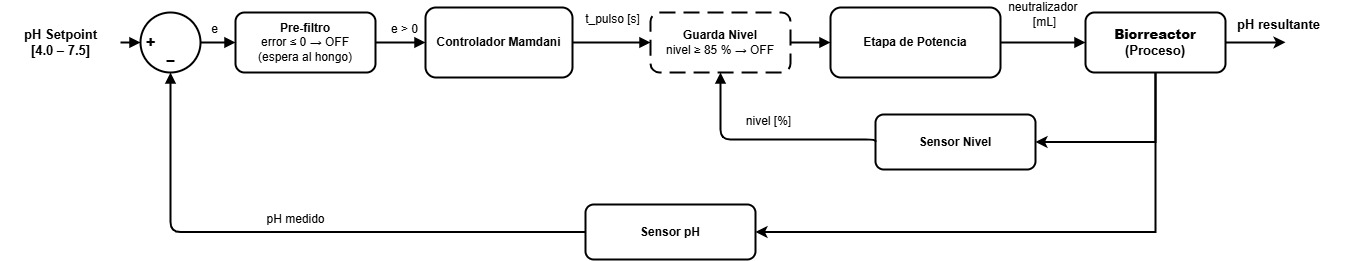
\includegraphics[width=0.9\textwidth]{Figuras/diagrama_control_pH.jpg}
  \caption{Diagrama de bloques del control de pH.}
  \label{fig:control_ph}
\end{figure}

El error se define como:
\begin{equation}
  e(t) = \text{pH}_{\text{setpoint}} - \text{pH}_{\text{actual}}
\end{equation}

El rango de control de interés es de 4 a 7.5 unidades de pH. La implementación
opera con un universo de entrada eficaz de $e \in [0, 0.8]$~pH: los errores
menores a la banda muerta ($e \leq 0.1$~pH) se cancelan mediante un prefiltro
y producen $t_\text{pulso} = 0$~s; los errores iguales o mayores al umbral de
saturación ($e \geq e_\text{sat} = 0.8$~pH) producen directamente el pulso máximo
$t_\text{p,máx} = 20$~s sin pasar por la inferencia.

La salida del inferenciador Mamdani es el tiempo de pulso normalizado
$t_\text{int} \in [0, 10]$~s, que se escala por el factor $k_\text{pulso} = 2$ para
obtener el tiempo de pulso efectivo $t_\text{pulso} = k_\text{pulso} \cdot t_\text{int}
\in [0, 20]$~s. Al operar la bomba a potencia fija, este tiempo determina el volumen
de neutralizador entregado en cada ciclo de control.

Se definieron cinco conjuntos difusos para cada variable a partir de la
caracterización experimental del pH (véase Cap.~\ref{cap:pruebas}). La
Figura~\ref{fig:mfs_difuso} muestra las funciones de membresía; la
Tabla~\ref{tab:mf_entrada} lista los parámetros de entrada y la
Tabla~\ref{tab:mf_salida} los de salida (universo interno $[0,10]$~s;
valores efectivos al multiplicar por $k_\text{pulso}=2$ en columna~Efectivo).

\begin{table}[H]
\centering
\caption{Funciones de membresía de la variable de entrada --- Error de pH.}
\label{tab:mf_entrada}
\renewcommand{\arraystretch}{1.3}
\small
\adjustbox{max width=\textwidth}{%
\begin{tabular}{lllllll}
\toprule
\textbf{Etiqueta} & \textbf{Nombre} & \textbf{Tipo} & \textbf{$a$} & \textbf{$b$} & \textbf{$c$} & \textbf{$d$} \\
\midrule
N   & Neutro            & trimf  & 0.00 & 0.00 & 0.06 & ---  \\
PE  & Error Pequeño     & trimf  & 0.04 & 0.15 & 0.28 & ---  \\
ME  & Error Medio       & trimf  & 0.22 & 0.35 & 0.50 & ---  \\
GE  & Error Grande      & trimf  & 0.42 & 0.58 & 0.75 & ---  \\
MG  & Error Muy Grande  & trapmf & 0.65 & 0.80 & 0.80 & 0.80 \\
\bottomrule
\end{tabular}
}
\end{table}

\begin{table}[H]
\centering
\caption{Funciones de membresía de la variable de salida --- Tiempo de pulso interno $t_\text{int}$ [s] y efectivo ($\times k_\text{pulso}=2$).}
\label{tab:mf_salida}
\renewcommand{\arraystretch}{1.3}
\small
\adjustbox{max width=\textwidth}{%
\begin{tabular}{lllllllll}
\toprule
\textbf{Etiq.} & \textbf{Nombre} & \textbf{Tipo} & \textbf{$a$} & \textbf{$b$} & \textbf{$c$} & \textbf{$d$} & \textbf{Efectivo (s)} & \textbf{Vol. aprox.} \\
\midrule
OFF   & Sin acci\'on    & trimf  & 0.0 & 0.0 &  1.5 & ---  & 0~s   & 0~mL \\
POCO  & Pulso corto     & trimf  & 3.0 & 5.0 &  7.0 & ---  & 10~s  & $\approx 390$~mL \\
MEDIO & Pulso medio     & trimf  & 5.5 & 7.0 &  9.0 & ---  & 14~s  & $\approx 546$~mL \\
MUCHO & Pulso largo     & trimf  & 7.5 & 9.0 & 10.0 & ---  & 18~s  & $\approx 702$~mL \\
MAX   & Pulso m\'aximo  & trapmf & 9.5 &10.0 & 10.0 & 10.0 & 20~s  & $\approx 780$~mL \\
\bottomrule
\end{tabular}
}
\end{table}

Las reglas que relacionan la magnitud del error con la acción de control se presentan
en la Tabla~\ref{tab:reglas_ph}. La inferencia es de tipo Mamdani y la defusificación se realiza
mediante el método de Centro de Gravedad (CoG), con un tiempo de muestreo
$T_s = 30$~s.

\begin{table}[H]
\centering
\caption{Base de reglas del controlador difuso de pH.}
\label{tab:reglas_ph}
\renewcommand{\arraystretch}{1.3}
\small
\begin{tabular}{clll}
\toprule
\textbf{Regla} & \textbf{Si error es\ldots} & \textbf{Entonces $t_{\text{pulso}}$ es\ldots} & \textbf{Volumen aprox.} \\
\midrule
1 & N  (Neutro)           & OFF   (0~s)    & 0~mL \\
2 & PE (Error Pequeño)    & POCO  (~10~s)  & $\approx 390$~mL \\
3 & ME (Error Medio)      & MEDIO (~14~s)  & $\approx 546$~mL \\
4 & GE (Error Grande)     & MUCHO (~18~s)  & $\approx 702$~mL \\
5 & MG (Error Muy Grande) & MAX   (20~s)\textsuperscript{*} & $\approx 780$~mL \\
\bottomrule
\end{tabular}
\end{table}

\noindent\textsuperscript{*}~La regla MG $\to$ MAX se implementa como saturación
directa al superar $e_\text{sat} = 0.8$~pH, sin pasar por el mecanismo de inferencia
Mamdani. La Figura~\ref{fig:superficie_control}b muestra la distribución de las
pruebas de validación por zona de operación, confirmando que los cinco escenarios
cubren las regiones PE, ME, GE y MG del espacio de control.

\begin{figure}[H]
  \centering
  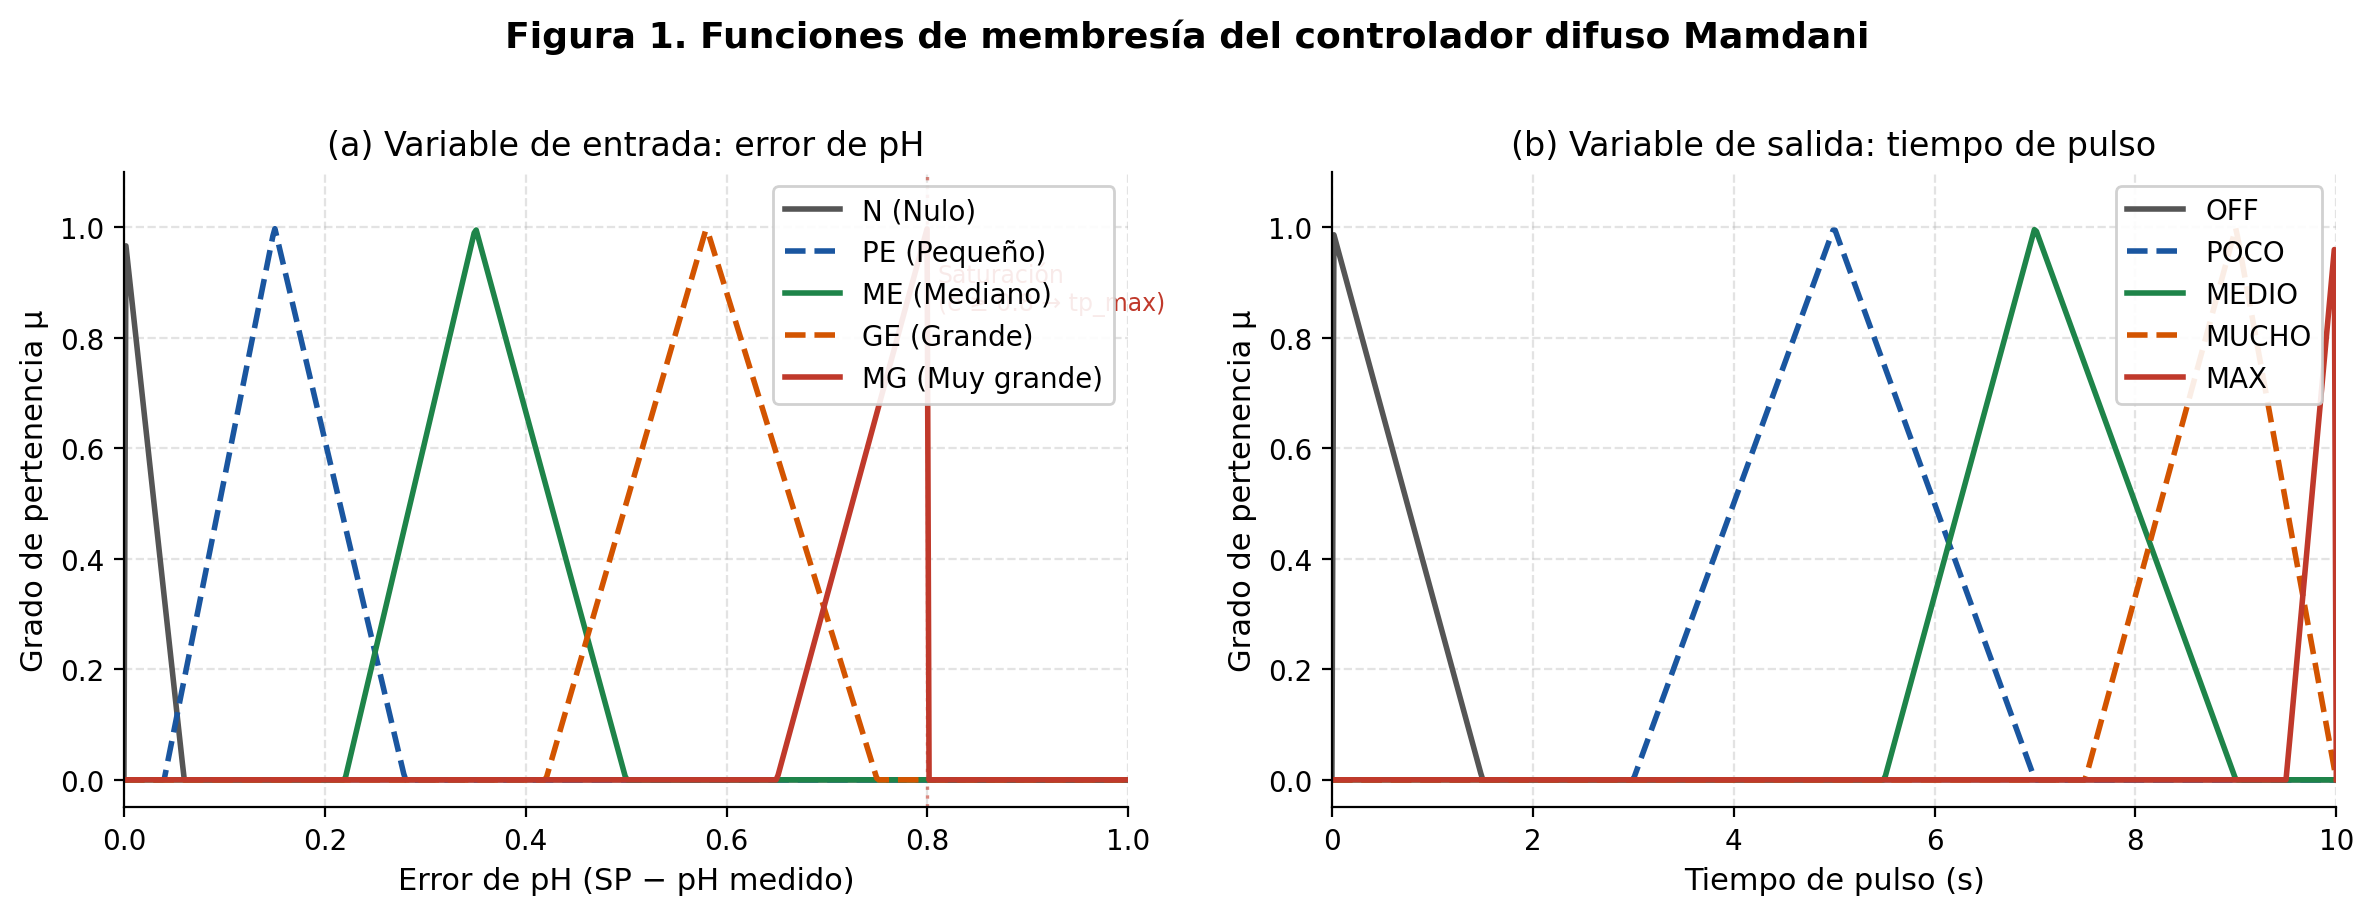
\includegraphics[width=\textwidth]{Figuras/fig_mfs_difuso.png}
  \caption{Funciones de membresía del controlador difuso Mamdani. (a) Variable de
           entrada: error de pH. (b) Variable de salida interna: tiempo de pulso en
           el universo $[0, 10]$~s antes de aplicar $k_\text{pulso}=2$.}
  \label{fig:mfs_difuso}
\end{figure}

\begin{figure}[H]
  \centering
  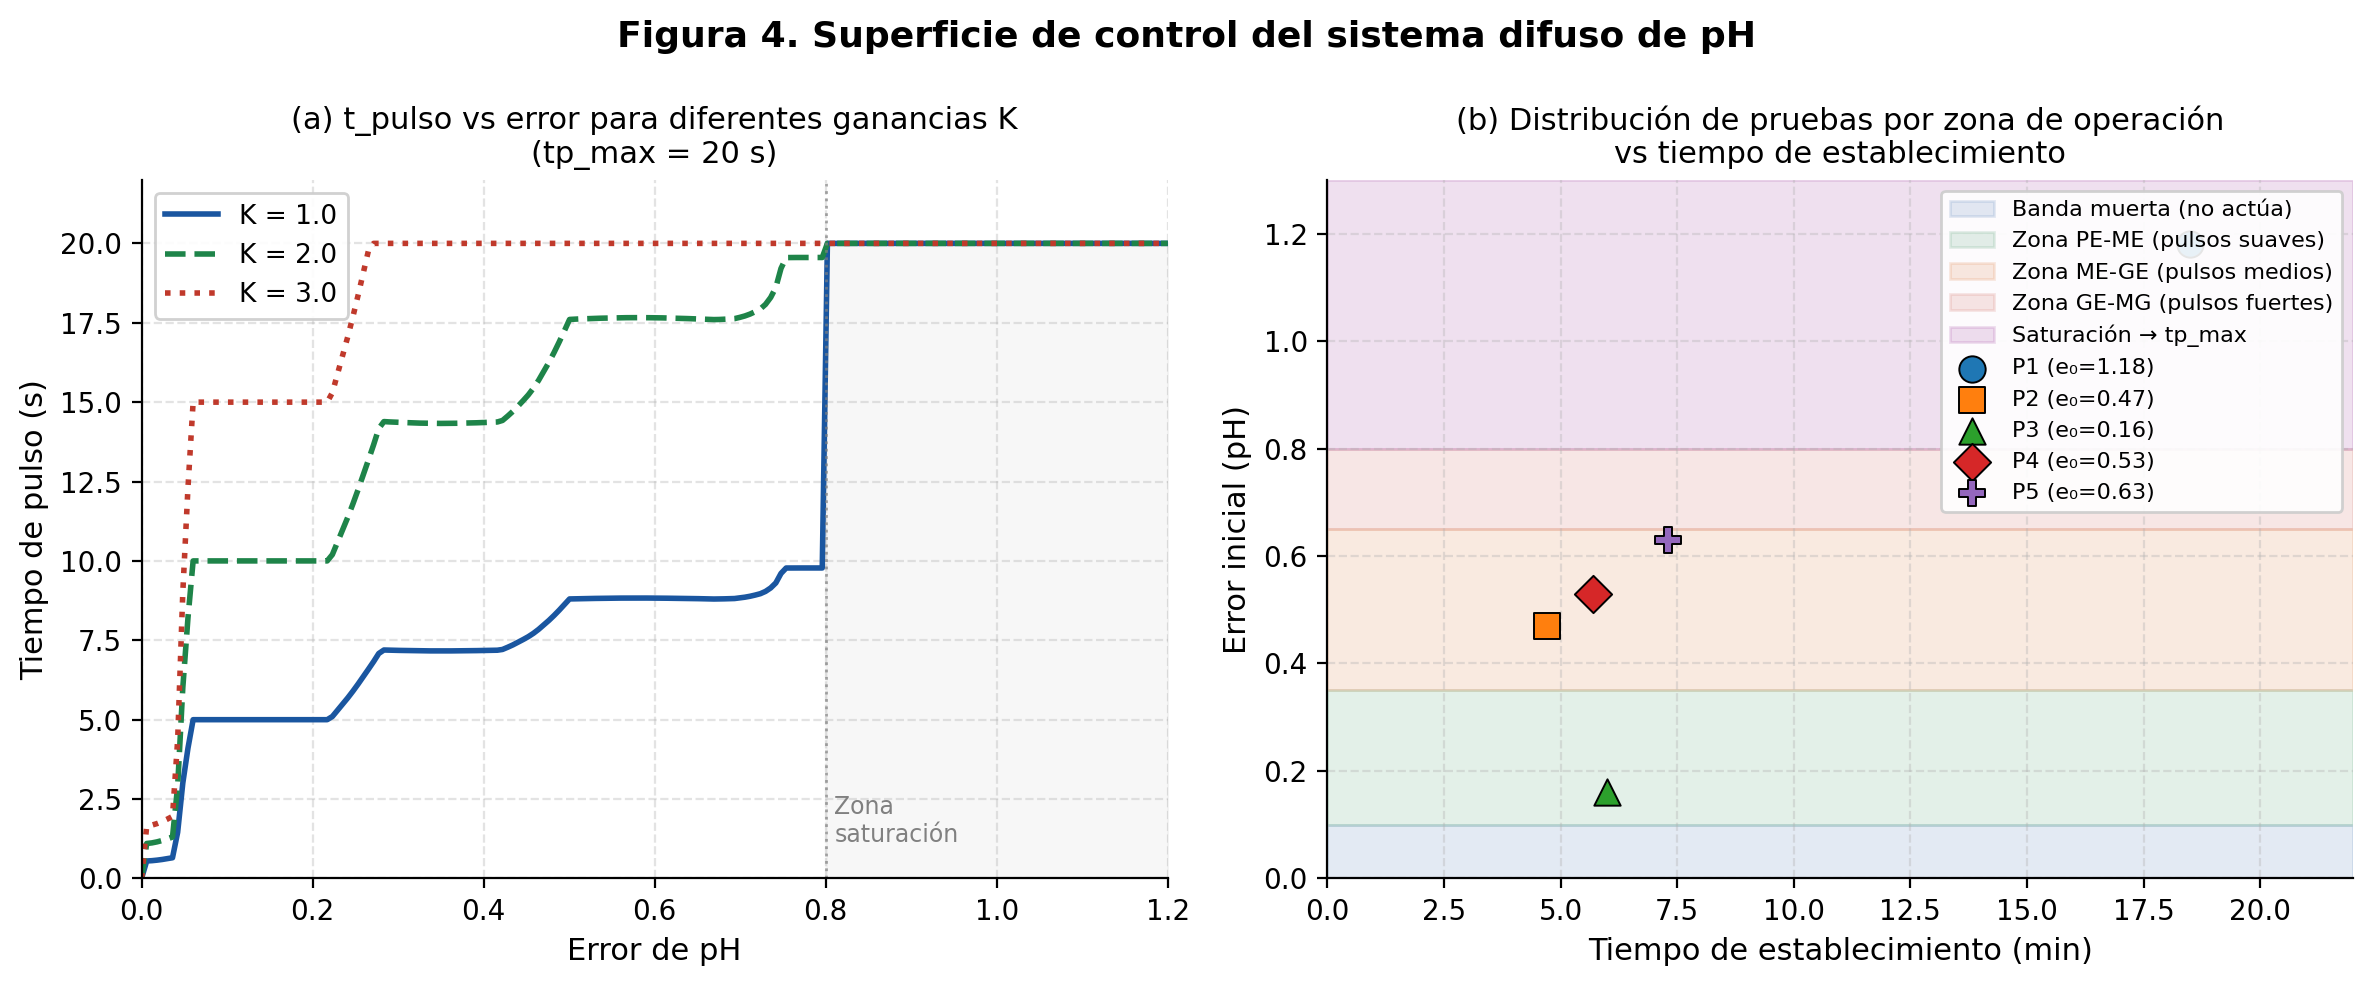
\includegraphics[width=\textwidth]{Figuras/fig_superficie_control.png}
  \caption{Superficie de control del sistema difuso de pH. (a) Tiempo de pulso interno
           vs.\ error de pH para diferentes valores del parámetro $K$. (b) Distribución
           de las pruebas de validación por zona de operación vs.\ tiempo de
           establecimiento.}
  \label{fig:superficie_control}
\end{figure}

\subsection{Control de nivel}

El control de pH opera incorporando volumen de contenido al tanque, por lo que es
necesario administrar el nivel de líquido para evitar desbordamientos. Para
gestionar el nivel de líquido se diseñó un lazo de control con histéresis. La lógica
de estados de este sistema opera de la siguiente manera:

\begin{enumerate}
  \item \textbf{Operación normal:} Si el nivel se encuentra por debajo del límite (95\%), el sistema opera con normalidad. Se habilita el control de pH.
  \item \textbf{Vaciado:} Si el nivel alcanza el 95\% de la capacidad total, se deshabilita el control de pH y se activa la bomba de drenado.
  \item \textbf{Histéresis:} El sistema vuelve a su operación habitual una vez que el nivel del tanque desciende del 85\%.
\end{enumerate}

Se cuenta con una banda de histéresis del 10\% para asegurar un tiempo suficiente
para la estabilización de la mezcla mediante el control de pH, así como para evitar
la oscilación continua de la bomba de drenado. La Figura~\ref{fig:control_nivel} muestra la lógica
de supervisión y control por histéresis del nivel.

\begin{figure}[H]
  \centering
  
\includegraphics[width=0.9\textwidth]{diagrama_control_nivel}
  \caption{Diagrama de control de nivel.}
  \label{fig:control_nivel}
\end{figure}

\subsection{Control de temperatura}

\subsubsection*{Dimensionamiento del actuador calefactor}

Se seleccionó un cable calefactor de carbono tipo 12K como actuador térmico.
Cada sección de manta emplea 4~m de cable con una resistividad lineal de
33~$\Omega$/m, distribuyendo seis bobinas alrededor del tanque. Los parámetros
eléctricos de cada bobina son:

\begin{align}
  R &= 33\;\Omega\text{/m} \times 4\;\text{m} = 132\;\Omega \notag \\
  I &= \frac{V}{R} = \frac{110\;\text{V}}{132\;\Omega} = 0.83\;\text{A} \notag \\
  P_\text{bobina} &= V \cdot I = 110\;\text{V} \times 0.83\;\text{A} = 91.3\;\text{W}
\end{align}

La potencia total instalada con las seis bobinas resulta:

\begin{equation}
  P_\text{total} = 6 \times 91.3\;\text{W} \approx 550\;\text{W}
\end{equation}

\subsubsection*{Cálculo de transferencia de calor}

Para estimar el tiempo de calentamiento se calculó la energía necesaria para
elevar la temperatura del agua y del acero inoxidable 304 desde
$T_1 = 18\,^{\circ}$C hasta $T_2 = 60\,^{\circ}$C
($\Delta T = 42\,^{\circ}$C), utilizando la ecuación de calor sensible
\cite{Cengel2015}:

\begin{equation}
  Q = m \cdot c_p \cdot \Delta T
  \label{eq:calor_sensible}
\end{equation}

\noindent\textbf{Masa de agua.} Con un volumen de operación de 55~L y
$\rho_\text{agua} = 1\,000\;\text{kg/m}^3$ \cite{Cengel2015}:
$m_\text{agua} = 55\;\text{kg}$.

\noindent\textbf{Masa del acero inoxidable 304.} Considerando el cuerpo
cilíndrico ($D_\text{int} = 21.5$~cm, $e = 3.5$~mm, $h = 1.035$~m) y las dos
tapas \cite{Cengel2015}:

\begin{align}
  V_\text{cil}  &= \pi h \!\left(r_\text{ext}^2 - r_\text{int}^2\right)
                 = \pi (1.035)(0.1110^2 - 0.1075^2) = 2.487 \times 10^{-3}\;\text{m}^3 \notag \\
  V_\text{tapas}&= 2\pi r_\text{ext}^2\, e
                 = 2\pi (0.1110)^2(0.0035) = 2.71 \times 10^{-4}\;\text{m}^3 \notag \\
  m_\text{acero}&= \rho_\text{acero}\,(V_\text{cil}+V_\text{tapas})
                 = 8\,000 \times 2.758 \times 10^{-3} = 22.06\;\text{kg}
\end{align}

\noindent\textbf{Energía total y tiempo de calentamiento.}
Con $c_{p,\text{agua}} = 4\,186\;\text{J/(kg·°C)}$ y
$c_{p,\text{acero}} = 500\;\text{J/(kg·°C)}$ \cite{Cengel2015}:

\begin{align}
  Q_\text{agua}  &= 55 \times 4\,186 \times 42 = 9\,669\,660\;\text{J} \notag \\
  Q_\text{acero} &= 22.06 \times 500 \times 42 = 463\,260\;\text{J} \notag \\
  Q_\text{total} &= 10\,132\,920\;\text{J}
\end{align}

\begin{equation}
  t = \frac{Q_\text{total}}{P_\text{total}} =
      \frac{10\,132\,920\;\text{J}}{550\;\text{W}} \approx 18\,423\;\text{s}
      \approx 5\;\text{h}\;7\;\text{min}
\end{equation}

\subsubsection*{Identificación de la planta y diseño del controlador PI}

El diseño del control de temperatura comenzó con la realización de una prueba a
lazo abierto aplicando un escalón unitario (fuente de calor constante) a un
recipiente con agua mientras se registró el cambio en la temperatura a lo largo del
tiempo con un sensor. La información recabada se utilizó para graficar la respuesta
transitoria de la planta (Figura~\ref{fig:planta_temp}).

\begin{figure}[H]
  \centering
  
\includegraphics[width=0.85\textwidth]{temp_planta_respuesta}
  \caption{Caracterización de la planta de temperatura: respuesta a lazo abierto ante escalón unitario de calor.}
  \label{fig:planta_temp}
\end{figure}

Al observar la gráfica de salida, se identificó un sistema de primer orden con
retardo, por lo que se pudo aproximar la planta utilizando la relación planteada por
Ziegler y Nichols:

\begin{equation}
G(s) = \frac{K e^{-Ls}}{\tau s + 1}
\end{equation}

Se determinaron además los parámetros $K = 20$, $L = 20$~s y $\tau = 1350$, los cuales
permitieron describir la planta y formular el control. La Figura~\ref{fig:respuesta_pid} muestra una
comparativa entre el comportamiento real del sistema, la planta aproximada y la
salida tras la aplicación del bloque de control PID.

\begin{figure}[H]
  \centering
  
\includegraphics[width=0.85\textwidth]{temp_validacion_pid}
  \caption{Validación del control PI ($K_p=0.017$, $\tau=1350$\,s): datos reales, planta aproximada en lazo abierto y respuesta PID.}
  \label{fig:respuesta_pid}
\end{figure}

Para la obtención de las constantes $K_p$ y $K_i$, el método de Ziegler-Nichols resultó
inestable y agresivo debido a que el retardo era despreciable en comparación con
su constante de tiempo ($\tau$). Por ello, se optó por el método de Asignación de Polos.
La ganancia proporcional se calculó utilizando el Criterio de Saturación al Arranque:

\begin{equation}
K_p = \frac{1}{\Delta T_{max}} = \frac{1}{60} = 0.0166 \approx 0.017
\end{equation}

Para el cálculo de la ganancia integral se igualó el Tiempo Integral ($\tau_i$) a la
Constante de Tiempo del proceso ($\tau$) para cancelar el polo dominante:

\begin{equation}
K_i = \frac{K_p}{\tau} = \frac{0.017}{1350} = 12.59 \times 10^{-6}
\end{equation}

La acción derivativa fue omitida debido a la naturaleza lenta de los procesos
térmicos. Por lo tanto, la función de transferencia del controlador puede
representarse como:

\begin{equation}
C(s) = 0.017 \cdot \frac{1350s + 1}{1350s}
\end{equation}

\begin{figure}[H]
  \centering
  
\includegraphics[width=0.85\textwidth]{temp_diagrama_bloques}
  \caption{Diagrama de bloques del sistema de control de temperatura en lazo cerrado.}
  \label{fig:bloques_temp}
\end{figure}

Donde $K_p = 0.017$ y $K_i = 12.59 \times 10^{-6}$.

\begin{figure}[H]
  \centering
  
\includegraphics[width=0.85\textwidth]{temp_simulacion_sp20}
  \caption{Simulación del sistema de control PI ante un escalón de $16.17\,^{\circ}$C a $20\,^{\circ}$C, con la potencia requerida al actuador.}
  \label{fig:sim_sp20}
\end{figure}

\section{Programación}

Para la realización del programa del biorreactor se tomó como base el diagrama de
la Figura~\ref{fig:flujo_simplificado} el cual muestra de manera sencilla los pasos generales que debe
realizar el programa.

\begin{figure}[H]
  \centering
  
\includegraphics[width=0.4\textwidth]{diagrama_flujo_simplificado}
  \caption{Diagrama de flujo simplificado de la programación del biorreactor.}
  \label{fig:flujo_simplificado}
\end{figure}

La Figura~\ref{fig:arquitectura_software} muestra la arquitectura completa del
software de la HMI, organizada en cinco capas: vista QML, backend C++,
controladores de lazo cerrado, drivers de hardware y hardware físico del
biorreactor, además del módulo de persistencia.

\begin{figure}[H]
  \centering
  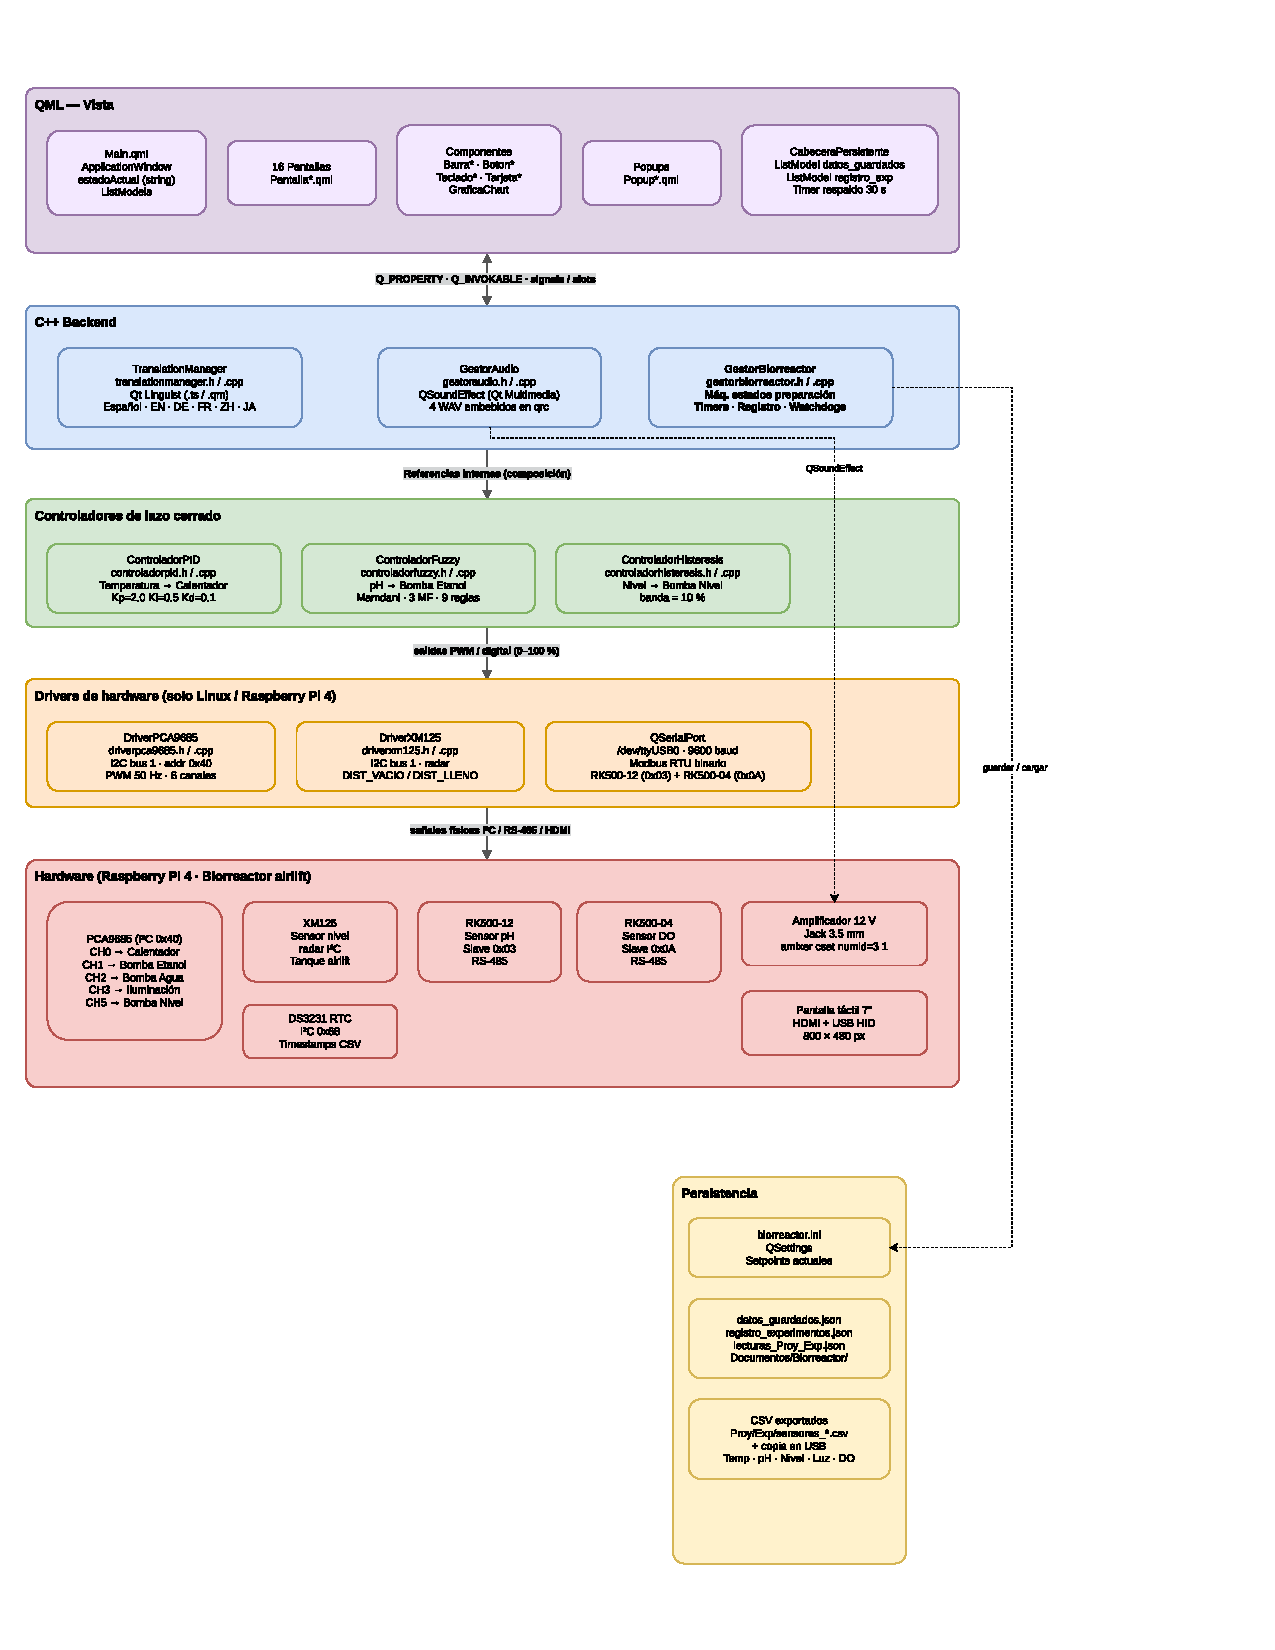
\includegraphics[width=1.2\textwidth, page=1]{Figuras/arquitectura_software.pdf}
  \caption{Arquitectura del software de control del biorreactor.}
  \label{fig:arquitectura_software}
\end{figure}

\section{Sistemas eléctricos}

En la Figura~\ref{fig:electr_conexiones}, se observa el esquema de conexiones eléctricas, en la que se contemplan el microcontrolador (Raspberry Pi 4B), los puertos para sensores (pH, O\textsubscript{2}, temperatura y nivel), así como las etapas de potencia, módulos de comunicación y fuente de alimentación.

\begin{figure}[H]
  \centering
  
\includegraphics[width=0.9\textwidth]{electr_diagrama_conexiones}
  \caption{Diagrama de conexiones eléctrico.}
  \label{fig:electr_conexiones}
\end{figure}

A continuación, en las Figuras~\ref{fig:electr_pistas}, \ref{fig:electr_superior} y~\ref{fig:electr_inferior} se muestran las pistas de la PCB, así como la vista final superior e inferior. En el Anexo~\ref{ap:especificaciones_electricas} se contienen los cálculos de potencia y consumos, así como la tabla de cableado con su respectivo calibre y finalmente una representación visual de conexiones para cada componente.

\begin{figure}[H]
  \centering
  
\includegraphics[width=0.9\textwidth]{electr_pistas_pcb}
  \caption{Pistas de la PCB.}
  \label{fig:electr_pistas}
\end{figure}

\begin{figure}[H]
  \centering
  
\includegraphics[width=0.9\textwidth]{electr_pcb_superior}
  \caption{Visualización superior de la PCB.}
  \label{fig:electr_superior}
\end{figure}

\begin{figure}[H]
  \centering
  
\includegraphics[width=0.9\textwidth]{electr_pcb_inferior}
  \caption{Visualización inferior de la PCB.}
  \label{fig:electr_inferior}
\end{figure}

\section{Plan de manufactura}

Para la fabricación de los elementos que se implementarán en el prototipo se ha decidido plantear un plan de manufactura. La Figura~\ref{fig:jerarquia_manufactura} muestra un diagrama que establece la jerarquía entre los distintos procesos necesarios para la creación del sistema.

\begin{figure}[H]
  \centering
  
\includegraphics[width=0.9\textwidth]{diagrama_jerarquia_manufactura}
  \caption{Diagrama de jerarquía para la manufactura del biorreactor.}
  \label{fig:jerarquia_manufactura}
\end{figure}

La información detallada sobre el plan de manufactura se muestra en el Apéndice~\ref{ap:manufactura}.

